\begin{frame}{La saturation}{Éviter les Accidents De Désaturation (ADD)}
Pendant que l'on est au fond
\begin{itemize}[<+->]
\item on respire de l'air sous pression
\item[$\Rightarrow$] on accumule de l'azote dans le corps.
\item Cet azote s'évacue à la remontée (dégazage).
\end{itemize}
\visible<3>{\begin{center}

\includegraphics[width=4cm]{ouverture-canette-boisson-gazeuse}
\end{center}}
\end{frame}

\begin{frame}{La remontée est maîtrisée}
\begin{block}{}
\begin{itemize}[<+->]
\item Remontée avec son guide de palanquée (moins vite que les plus petites bulles);
\item éventuellement faire des paliers;
\item rester dans des profils de plongée sécuritaires (\emph{c.f.} courbe sans palier obligatoire).
\end{itemize}
\end{block}
\end{frame}

\begin{frame}{Facteurs favorisants}
Attention, ces accidents dépendent:
\begin{itemize}[<+(1)->]
\item de l'individu,
\item de l'état de santé général (obésité, cigarette, \dots), de l'âge (plus de 40 ans),
\item de l'état de forme physique et morale (manque de sommeil, stress, \dots).
\end{itemize}
\end{frame}

\begin{frame}{Signes}
\juxt{%
\begin{itemize}
\item Douleurs, 
\item fourmillements,
\item grande fatigue,
\item maux de tête,
\item vertiges,
\item nausées,
\item vomissements\dots
\end{itemize}
}{%
\begin{alertblock}<2>{}
\danger{En cas de doute on se signale}
\end{alertblock}
}
\end{frame}

\begin{frame}{Courbe de plongée sans palier obligatoire}
\centering\includegraphics[height=6cm]{courbe_secu}
\end{frame}

\zap{ %% »
\begin{frame}{C'est quoi trop profond, c'est combien trop longtemps?}
{1\up{ère} réponse: les tables MN90. Le principe}
\begin{itemize}[<+->]
\item Pour un temps à une profondeur, elles donnent les paliers à respecter,
  sous hypothèse:
  \begin{itemize}
  \item profil carré,
  \item vitesse de remontée entre 15 et 17 m/min.
  \end{itemize}
\item[$\Rightarrow$] La profondeur max donne le temps sans palier et les paliers à respecter
  le cas échéant.
  Les tables donnent aussi l'état de saturation à la fin de la plongée.\\
  $\Rightarrow$ État de saturation au démarrage de la plongée suivante.
\end{itemize}
\end{frame}

\begin{frame}{C'est quoi trop profond, c'est combien trop longtemps?}
{1\up{ère} réponse: les tables MN90. Un exemple}
\begin{itemize}[<+->]
\item Première plongée le matin, 35 min à 20 mètres max, sortie à 11h25.
\item[$\Rightarrow$] Pas de paliers, groupe de saturation E.
\item Deuxième plongée l'après-midi, à 14h15, 40 min à 15 mètres max.
\item[$\Rightarrow$] 2h50 de temps entre les plongées,
\item[$\Rightarrow$] 13 minutes de pénalisation à ajouter,
\item[$\Rightarrow$] 53 minutes à 15 mètres, pas de palier.
\end{itemize}
\end{frame}

\begin{frame}{C'est quoi trop profond, c'est combien trop longtemps?}
{1\up{ère} réponse: les tables MN90. Dans la pratique}
Elles sont peu utilisées, le profil carré n'est pas réaliste, mais il reste
sécuritaire.

Elles nécessitent de se tenir dans le détail aux caractéristiques 
prévues de la plongée, avec peu de capacité d'adaptation, recalculer sous
l'eau n'est pas simple!
\end{frame}

\begin{frame}{C'est quoi trop profond, c'est combien trop longtemps?}
{2\up{nde} réponse: un ordinateur de plongée.}
\only<1>{Plus fin que les tables, prend en compte le profil réel de la plongée
et calcule en temps réel. Permet de comparer le profil réel au profil prévu,
permet d'être adaptable.}
\only<2->{\begin{alertblock}{ATTENTION}
Être adaptable ne signifie pas ne pas respecter les paramètres de
plongée établis par le DP!
\only<3->{%

Un ordinateur n'est pas parole d'évangile, il faut le comprendre pour l'utiliser.
Il faut savoir le paramétrer, savoir sous quels paramètres il est actif, et
\emph{ne pas changer d'ordinateur entre deux plongées successives!}}
\end{alertblock}}
\visible<4>{\centering\large Lire le manuel d'utilisation!}
\end{frame}

\begin{frame}{C'est quoi trop profond, c'est combien trop longtemps?}
{2\up{nde} réponse: un ordinateur de plongée. Quoi ça raconte?}
\begin{minipage}{0.48\textwidth}
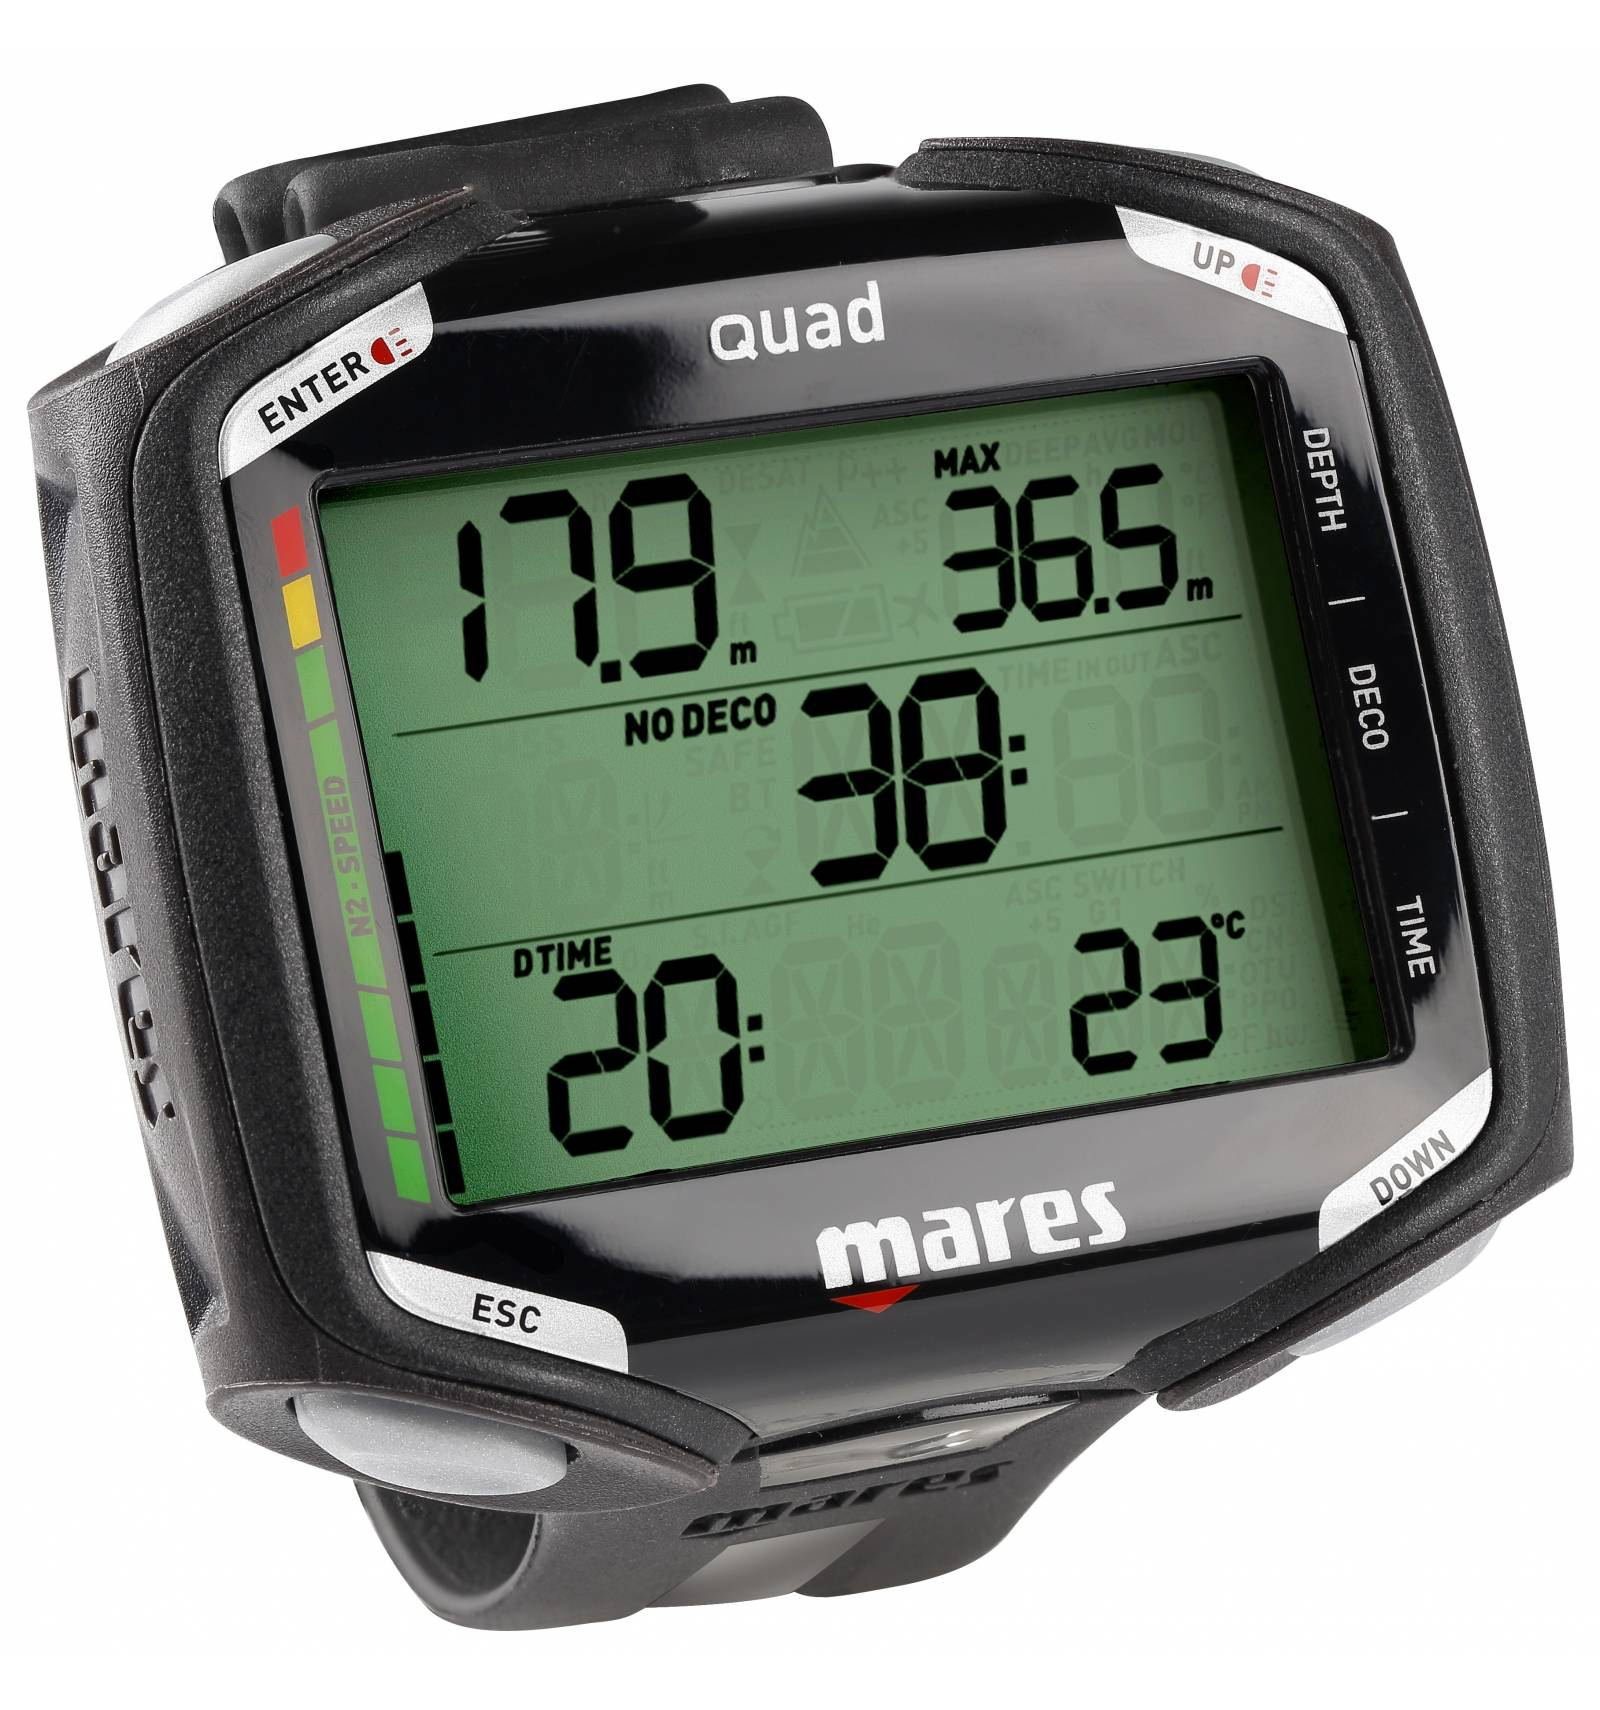
\includegraphics[width=\textwidth]{ordinateur-quad-mares}
\end{minipage}\hfill
\begin{minipage}{0.48\textwidth}
\only<-7>{%
\begin{itemize}[<+->]
\item Profondeur courante,
\item profondeur max,
\item temps de plongée,
\item temps sans palier/paliers à effectuer,
\item mélange utilisé (air, nitrox,\dots),
\item vitesse de remontée,
\item \dots
\end{itemize}}
\only<8>{%
\begin{center}
Il faut lire le manuel de l'ordinateur.
\end{center}
}
\end{minipage}
\end{frame}

} %% end zap «
